\documentclass[11pt]{amsart}
\usepackage{aurical}
%\usepackage{ccfonts} % this sets the fonts for tics in figures and equations.
\usepackage[T1]{fontenc}
\renewcommand*{\familydefault}{AuriocusKalligraphicus}
%\renewcommand*{\rmdefault}{AuriocusKalligraphicus}
%\renewcommand*{\sfdefault}{AuriocusKalligraphicus}

\usepackage{geometry}                % See geometry.pdf to learn the layout options. There are lots.
\geometry{letterpaper}                   % ... or a4paper or a5paper or ... 
%\geometry{landscape}                % Activate for for rotated page geometry
%\usepackage[parfill]{parskip}    % Activate to begin paragraphs with an empty line rather than an indent
\usepackage{graphicx}
\usepackage{amssymb}
\usepackage{epstopdf}
\usepackage{color}
\usepackage{multicol}

\DeclareGraphicsRule{.tif}{png}{.png}{`convert #1 `dirname #1`/`basename #1 .tif`.png}

\title{Figures and fonts matching Journal guidelines with Gnuplot.jl}
\author{Lazaro Alonso}
%\date{}                                           % Activate to display a given date or no date

\begin{document}
\maketitle
%\begin{multicols}{2}
What happens if we write some equations here? what would be the family font?

\begin{equation}
\frac{1}{2\pi i} \int_{\gamma} f = \sum_{k=1}^{m} n(\gamma; a_{k}) Res(f; a_{k}).
\end{equation}

\begin{figure}
\resizebox{.48\linewidth}{!}{% GNUPLOT: LaTeX picture with Postscript
\begingroup
  \makeatletter
  \providecommand\color[2][]{%
    \GenericError{(gnuplot) \space\space\space\@spaces}{%
      Package color not loaded in conjunction with
      terminal option `colourtext'%
    }{See the gnuplot documentation for explanation.%
    }{Either use 'blacktext' in gnuplot or load the package
      color.sty in LaTeX.}%
    \renewcommand\color[2][]{}%
  }%
  \providecommand\includegraphics[2][]{%
    \GenericError{(gnuplot) \space\space\space\@spaces}{%
      Package graphicx or graphics not loaded%
    }{See the gnuplot documentation for explanation.%
    }{The gnuplot epslatex terminal needs graphicx.sty or graphics.sty.}%
    \renewcommand\includegraphics[2][]{}%
  }%
  \providecommand\rotatebox[2]{#2}%
  \@ifundefined{ifGPcolor}{%
    \newif\ifGPcolor
    \GPcolortrue
  }{}%
  \@ifundefined{ifGPblacktext}{%
    \newif\ifGPblacktext
    \GPblacktexttrue
  }{}%
  % define a \g@addto@macro without @ in the name:
  \let\gplgaddtomacro\g@addto@macro
  % define empty templates for all commands taking text:
  \gdef\gplbacktext{}%
  \gdef\gplfronttext{}%
  \makeatother
  \ifGPblacktext
    % no textcolor at all
    \def\colorrgb#1{}%
    \def\colorgray#1{}%
  \else
    % gray or color?
    \ifGPcolor
      \def\colorrgb#1{\color[rgb]{#1}}%
      \def\colorgray#1{\color[gray]{#1}}%
      \expandafter\def\csname LTw\endcsname{\color{white}}%
      \expandafter\def\csname LTb\endcsname{\color{black}}%
      \expandafter\def\csname LTa\endcsname{\color{black}}%
      \expandafter\def\csname LT0\endcsname{\color[rgb]{1,0,0}}%
      \expandafter\def\csname LT1\endcsname{\color[rgb]{0,1,0}}%
      \expandafter\def\csname LT2\endcsname{\color[rgb]{0,0,1}}%
      \expandafter\def\csname LT3\endcsname{\color[rgb]{1,0,1}}%
      \expandafter\def\csname LT4\endcsname{\color[rgb]{0,1,1}}%
      \expandafter\def\csname LT5\endcsname{\color[rgb]{1,1,0}}%
      \expandafter\def\csname LT6\endcsname{\color[rgb]{0,0,0}}%
      \expandafter\def\csname LT7\endcsname{\color[rgb]{1,0.3,0}}%
      \expandafter\def\csname LT8\endcsname{\color[rgb]{0.5,0.5,0.5}}%
    \else
      % gray
      \def\colorrgb#1{\color{black}}%
      \def\colorgray#1{\color[gray]{#1}}%
      \expandafter\def\csname LTw\endcsname{\color{white}}%
      \expandafter\def\csname LTb\endcsname{\color{black}}%
      \expandafter\def\csname LTa\endcsname{\color{black}}%
      \expandafter\def\csname LT0\endcsname{\color{black}}%
      \expandafter\def\csname LT1\endcsname{\color{black}}%
      \expandafter\def\csname LT2\endcsname{\color{black}}%
      \expandafter\def\csname LT3\endcsname{\color{black}}%
      \expandafter\def\csname LT4\endcsname{\color{black}}%
      \expandafter\def\csname LT5\endcsname{\color{black}}%
      \expandafter\def\csname LT6\endcsname{\color{black}}%
      \expandafter\def\csname LT7\endcsname{\color{black}}%
      \expandafter\def\csname LT8\endcsname{\color{black}}%
    \fi
  \fi
    \setlength{\unitlength}{0.0500bp}%
    \ifx\gptboxheight\undefined%
      \newlength{\gptboxheight}%
      \newlength{\gptboxwidth}%
      \newsavebox{\gptboxtext}%
    \fi%
    \setlength{\fboxrule}{0.5pt}%
    \setlength{\fboxsep}{1pt}%
    \definecolor{tbcol}{rgb}{1,1,1}%
\begin{picture}(7200.00,4740.00)%
    \gplgaddtomacro\gplbacktext{%
    }%
    \gplgaddtomacro\gplfronttext{%
      \csname LTb\endcsname%%
      \put(161,2377){\rotatebox{-270}{\makebox(0,0){\strut{}ylabel $x$}}}%
      \csname LTb\endcsname%%
      \put(3849,123){\makebox(0,0){\strut{}xlabel $f(x)$ }}%
      \csname LTb\endcsname%%
      \put(3911,4033){\makebox(0,0)[r]{\strut{}$n=0$}}%
      \csname LTb\endcsname%%
      \put(3911,3858){\makebox(0,0)[r]{\strut{}$n=1$}}%
      \csname LTb\endcsname%%
      \put(3911,3682){\makebox(0,0)[r]{\strut{}$n=2$}}%
      \csname LTb\endcsname%%
      \put(3911,3506){\makebox(0,0)[r]{\strut{}$n=3$}}%
      \csname LTb\endcsname%%
      \put(3911,3330){\makebox(0,0)[r]{\strut{}\footnotesize $sin(x)$}}%
      \csname LTb\endcsname%%
      \put(714,562){\makebox(0,0)[r]{\strut{}$-1.5$}}%
      \csname LTb\endcsname%%
      \put(714,1167){\makebox(0,0)[r]{\strut{}$-1$}}%
      \csname LTb\endcsname%%
      \put(714,1772){\makebox(0,0)[r]{\strut{}$-0.5$}}%
      \csname LTb\endcsname%%
      \put(714,2377){\makebox(0,0)[r]{\strut{}$0$}}%
      \csname LTb\endcsname%%
      \put(714,2982){\makebox(0,0)[r]{\strut{}$0.5$}}%
      \csname LTb\endcsname%%
      \put(714,3587){\makebox(0,0)[r]{\strut{}$1$}}%
      \csname LTb\endcsname%%
      \put(714,4192){\makebox(0,0)[r]{\strut{}$1.5$}}%
      \csname LTb\endcsname%%
      \put(1338,386){\makebox(0,0){\strut{}$-\pi$}}%
      \csname LTb\endcsname%%
      \put(2593,386){\makebox(0,0){\strut{}$-\pi/2$}}%
      \csname LTb\endcsname%%
      \put(3849,386){\makebox(0,0){\strut{}$0$}}%
      \csname LTb\endcsname%%
      \put(5104,386){\makebox(0,0){\strut{}$\pi/2$}}%
      \csname LTb\endcsname%%
      \put(6360,386){\makebox(0,0){\strut{}$\pi$}}%
      \csname LTb\endcsname%%
      \put(4578,1288){\makebox(0,0){\strut{}\begin{minipage}[c]{\textwidth}\begin{equation*}\sin(x) = \sum_0^{+\infty} \frac{(-1)^n}{(2n + 1)!} x^{2n+1}\end{equation*} \end{minipage}}}%
      \csname LTb\endcsname%%
      \put(3849,4456){\makebox(0,0){\strut{}Title: Polynomial approximation of sin(x)}}%
    }%
    \gplbacktext
    \put(0,0){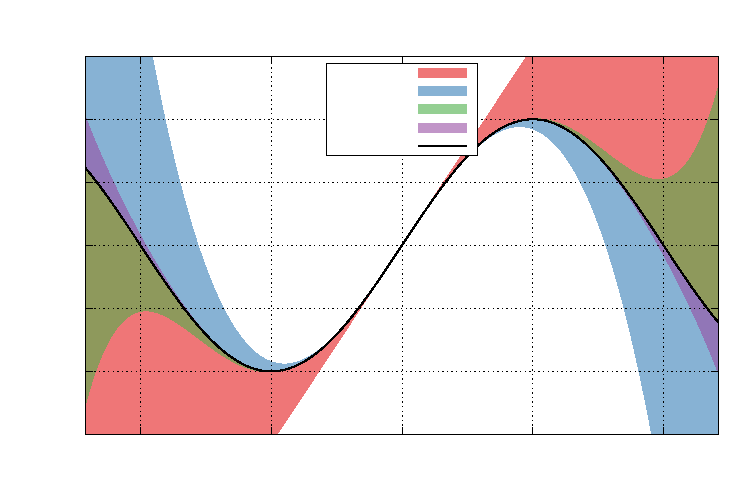
\includegraphics[width={360.00bp},height={237.00bp}]{test}}%
    \gplfronttext
  \end{picture}%
\endgroup
}
\resizebox{.48\linewidth}{!}{% GNUPLOT: LaTeX picture with Postscript
\begingroup
  \makeatletter
  \providecommand\color[2][]{%
    \GenericError{(gnuplot) \space\space\space\@spaces}{%
      Package color not loaded in conjunction with
      terminal option `colourtext'%
    }{See the gnuplot documentation for explanation.%
    }{Either use 'blacktext' in gnuplot or load the package
      color.sty in LaTeX.}%
    \renewcommand\color[2][]{}%
  }%
  \providecommand\includegraphics[2][]{%
    \GenericError{(gnuplot) \space\space\space\@spaces}{%
      Package graphicx or graphics not loaded%
    }{See the gnuplot documentation for explanation.%
    }{The gnuplot epslatex terminal needs graphicx.sty or graphics.sty.}%
    \renewcommand\includegraphics[2][]{}%
  }%
  \providecommand\rotatebox[2]{#2}%
  \@ifundefined{ifGPcolor}{%
    \newif\ifGPcolor
    \GPcolortrue
  }{}%
  \@ifundefined{ifGPblacktext}{%
    \newif\ifGPblacktext
    \GPblacktexttrue
  }{}%
  % define a \g@addto@macro without @ in the name:
  \let\gplgaddtomacro\g@addto@macro
  % define empty templates for all commands taking text:
  \gdef\gplbacktext{}%
  \gdef\gplfronttext{}%
  \makeatother
  \ifGPblacktext
    % no textcolor at all
    \def\colorrgb#1{}%
    \def\colorgray#1{}%
  \else
    % gray or color?
    \ifGPcolor
      \def\colorrgb#1{\color[rgb]{#1}}%
      \def\colorgray#1{\color[gray]{#1}}%
      \expandafter\def\csname LTw\endcsname{\color{white}}%
      \expandafter\def\csname LTb\endcsname{\color{black}}%
      \expandafter\def\csname LTa\endcsname{\color{black}}%
      \expandafter\def\csname LT0\endcsname{\color[rgb]{1,0,0}}%
      \expandafter\def\csname LT1\endcsname{\color[rgb]{0,1,0}}%
      \expandafter\def\csname LT2\endcsname{\color[rgb]{0,0,1}}%
      \expandafter\def\csname LT3\endcsname{\color[rgb]{1,0,1}}%
      \expandafter\def\csname LT4\endcsname{\color[rgb]{0,1,1}}%
      \expandafter\def\csname LT5\endcsname{\color[rgb]{1,1,0}}%
      \expandafter\def\csname LT6\endcsname{\color[rgb]{0,0,0}}%
      \expandafter\def\csname LT7\endcsname{\color[rgb]{1,0.3,0}}%
      \expandafter\def\csname LT8\endcsname{\color[rgb]{0.5,0.5,0.5}}%
    \else
      % gray
      \def\colorrgb#1{\color{black}}%
      \def\colorgray#1{\color[gray]{#1}}%
      \expandafter\def\csname LTw\endcsname{\color{white}}%
      \expandafter\def\csname LTb\endcsname{\color{black}}%
      \expandafter\def\csname LTa\endcsname{\color{black}}%
      \expandafter\def\csname LT0\endcsname{\color{black}}%
      \expandafter\def\csname LT1\endcsname{\color{black}}%
      \expandafter\def\csname LT2\endcsname{\color{black}}%
      \expandafter\def\csname LT3\endcsname{\color{black}}%
      \expandafter\def\csname LT4\endcsname{\color{black}}%
      \expandafter\def\csname LT5\endcsname{\color{black}}%
      \expandafter\def\csname LT6\endcsname{\color{black}}%
      \expandafter\def\csname LT7\endcsname{\color{black}}%
      \expandafter\def\csname LT8\endcsname{\color{black}}%
    \fi
  \fi
    \setlength{\unitlength}{0.0500bp}%
    \ifx\gptboxheight\undefined%
      \newlength{\gptboxheight}%
      \newlength{\gptboxwidth}%
      \newsavebox{\gptboxtext}%
    \fi%
    \setlength{\fboxrule}{0.5pt}%
    \setlength{\fboxsep}{1pt}%
    \definecolor{tbcol}{rgb}{1,1,1}%
\begin{picture}(7200.00,4740.00)%
      \csname LTb\endcsname%%
      \put(3590,4544){\makebox(0,0){\strut{}Interlocking Tori}}%
    \gplgaddtomacro\gplbacktext{%
    }%
    \gplgaddtomacro\gplfronttext{%
      \csname LTb\endcsname%%
      \put(359,296){\makebox(0,0){\strut{}$-1.5$}}%
      \csname LTb\endcsname%%
      \put(837,296){\makebox(0,0){\strut{}$-1$}}%
      \csname LTb\endcsname%%
      \put(1316,296){\makebox(0,0){\strut{}$-0.5$}}%
      \csname LTb\endcsname%%
      \put(1795,296){\makebox(0,0){\strut{}$0$}}%
      \csname LTb\endcsname%%
      \put(2273,296){\makebox(0,0){\strut{}$0.5$}}%
      \csname LTb\endcsname%%
      \put(2752,296){\makebox(0,0){\strut{}$1$}}%
      \csname LTb\endcsname%%
      \put(3231,296){\makebox(0,0){\strut{}$1.5$}}%
      \csname LTb\endcsname%%
      \put(1795,0){\makebox(0,0){\strut{}$z$ dense}}%
      \csname LTb\endcsname%%
      \put(1830,3906){\makebox(0,0){\strut{}PM3D surface}}%
      \put(1830,3730){\makebox(0,0){\strut{}no depth sorting}}%
    }%
    \gplgaddtomacro\gplbacktext{%
    }%
    \gplgaddtomacro\gplfronttext{%
      \csname LTb\endcsname%%
      \put(6703,708){\makebox(0,0)[l]{\strut{}$-1.5$}}%
      \csname LTb\endcsname%%
      \put(6703,1101){\makebox(0,0)[l]{\strut{}$-1$}}%
      \csname LTb\endcsname%%
      \put(6703,1494){\makebox(0,0)[l]{\strut{}$-0.5$}}%
      \csname LTb\endcsname%%
      \put(6703,1888){\makebox(0,0)[l]{\strut{}$0$}}%
      \csname LTb\endcsname%%
      \put(6703,2281){\makebox(0,0)[l]{\strut{}$0.5$}}%
      \csname LTb\endcsname%%
      \put(6703,2674){\makebox(0,0)[l]{\strut{}$1$}}%
      \csname LTb\endcsname%%
      \put(6703,3068){\makebox(0,0)[l]{\strut{}$1.5$}}%
      \csname LTb\endcsname%%
      \put(7144,1888){\rotatebox{-270}{\makebox(0,0){\strut{}$z$}}}%
      \csname LTb\endcsname%%
      \put(4846,3906){\makebox(0,0){\strut{}PM3D surface}}%
      \put(4846,3730){\makebox(0,0){\strut{}depth sorting}}%
    }%
    \gplbacktext
    \put(0,0){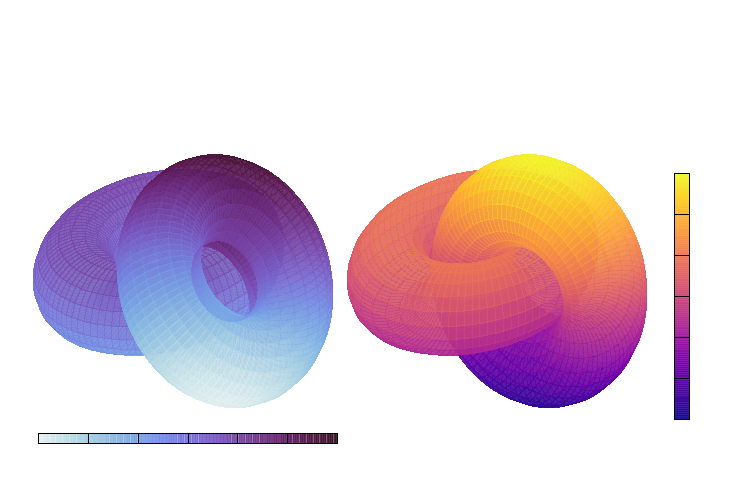
\includegraphics[width={360.00bp},height={237.00bp}]{test_torus}}%
    \gplfronttext
  \end{picture}%
\endgroup
}

  \caption{Here it goes our nice caption explaining what all colours and lines are about. Note the mix of normal text and
  \LaTeX -like equations fonts.}
\end{figure}

\begin{figure}
  \resizebox{.48\linewidth}{!}{% GNUPLOT: LaTeX picture with Postscript
\begingroup
  \makeatletter
  \providecommand\color[2][]{%
    \GenericError{(gnuplot) \space\space\space\@spaces}{%
      Package color not loaded in conjunction with
      terminal option `colourtext'%
    }{See the gnuplot documentation for explanation.%
    }{Either use 'blacktext' in gnuplot or load the package
      color.sty in LaTeX.}%
    \renewcommand\color[2][]{}%
  }%
  \providecommand\includegraphics[2][]{%
    \GenericError{(gnuplot) \space\space\space\@spaces}{%
      Package graphicx or graphics not loaded%
    }{See the gnuplot documentation for explanation.%
    }{The gnuplot epslatex terminal needs graphicx.sty or graphics.sty.}%
    \renewcommand\includegraphics[2][]{}%
  }%
  \providecommand\rotatebox[2]{#2}%
  \@ifundefined{ifGPcolor}{%
    \newif\ifGPcolor
    \GPcolortrue
  }{}%
  \@ifundefined{ifGPblacktext}{%
    \newif\ifGPblacktext
    \GPblacktexttrue
  }{}%
  % define a \g@addto@macro without @ in the name:
  \let\gplgaddtomacro\g@addto@macro
  % define empty templates for all commands taking text:
  \gdef\gplbacktext{}%
  \gdef\gplfronttext{}%
  \makeatother
  \ifGPblacktext
    % no textcolor at all
    \def\colorrgb#1{}%
    \def\colorgray#1{}%
  \else
    % gray or color?
    \ifGPcolor
      \def\colorrgb#1{\color[rgb]{#1}}%
      \def\colorgray#1{\color[gray]{#1}}%
      \expandafter\def\csname LTw\endcsname{\color{white}}%
      \expandafter\def\csname LTb\endcsname{\color{black}}%
      \expandafter\def\csname LTa\endcsname{\color{black}}%
      \expandafter\def\csname LT0\endcsname{\color[rgb]{1,0,0}}%
      \expandafter\def\csname LT1\endcsname{\color[rgb]{0,1,0}}%
      \expandafter\def\csname LT2\endcsname{\color[rgb]{0,0,1}}%
      \expandafter\def\csname LT3\endcsname{\color[rgb]{1,0,1}}%
      \expandafter\def\csname LT4\endcsname{\color[rgb]{0,1,1}}%
      \expandafter\def\csname LT5\endcsname{\color[rgb]{1,1,0}}%
      \expandafter\def\csname LT6\endcsname{\color[rgb]{0,0,0}}%
      \expandafter\def\csname LT7\endcsname{\color[rgb]{1,0.3,0}}%
      \expandafter\def\csname LT8\endcsname{\color[rgb]{0.5,0.5,0.5}}%
    \else
      % gray
      \def\colorrgb#1{\color{black}}%
      \def\colorgray#1{\color[gray]{#1}}%
      \expandafter\def\csname LTw\endcsname{\color{white}}%
      \expandafter\def\csname LTb\endcsname{\color{black}}%
      \expandafter\def\csname LTa\endcsname{\color{black}}%
      \expandafter\def\csname LT0\endcsname{\color{black}}%
      \expandafter\def\csname LT1\endcsname{\color{black}}%
      \expandafter\def\csname LT2\endcsname{\color{black}}%
      \expandafter\def\csname LT3\endcsname{\color{black}}%
      \expandafter\def\csname LT4\endcsname{\color{black}}%
      \expandafter\def\csname LT5\endcsname{\color{black}}%
      \expandafter\def\csname LT6\endcsname{\color{black}}%
      \expandafter\def\csname LT7\endcsname{\color{black}}%
      \expandafter\def\csname LT8\endcsname{\color{black}}%
    \fi
  \fi
    \setlength{\unitlength}{0.0500bp}%
    \ifx\gptboxheight\undefined%
      \newlength{\gptboxheight}%
      \newlength{\gptboxwidth}%
      \newsavebox{\gptboxtext}%
    \fi%
    \setlength{\fboxrule}{0.5pt}%
    \setlength{\fboxsep}{1pt}%
    \definecolor{tbcol}{rgb}{1,1,1}%
\begin{picture}(7200.00,4740.00)%
    \gplgaddtomacro\gplbacktext{%
      \csname LTb\endcsname%%
      \put(1373,1057){\makebox(0,0)[r]{\strut{}$-4$}}%
      \csname LTb\endcsname%%
      \put(1373,1717){\makebox(0,0)[r]{\strut{}$-2$}}%
      \csname LTb\endcsname%%
      \put(1373,2377){\makebox(0,0)[r]{\strut{}$0$}}%
      \csname LTb\endcsname%%
      \put(1373,3037){\makebox(0,0)[r]{\strut{}$2$}}%
      \csname LTb\endcsname%%
      \put(1373,3697){\makebox(0,0)[r]{\strut{}$4$}}%
      \csname LTb\endcsname%%
      \put(1966,386){\makebox(0,0){\strut{}$-4$}}%
      \csname LTb\endcsname%%
      \put(2626,386){\makebox(0,0){\strut{}$-2$}}%
      \csname LTb\endcsname%%
      \put(3286,386){\makebox(0,0){\strut{}$0$}}%
      \csname LTb\endcsname%%
      \put(3946,386){\makebox(0,0){\strut{}$2$}}%
      \csname LTb\endcsname%%
      \put(4605,386){\makebox(0,0){\strut{}$4$}}%
    }%
    \gplgaddtomacro\gplfronttext{%
      \csname LTb\endcsname%%
      \put(1016,2377){\rotatebox{-270}{\makebox(0,0){\strut{}$y$}}}%
      \csname LTb\endcsname%%
      \put(3286,123){\makebox(0,0){\strut{}$x$}}%
      \csname LTb\endcsname%%
      \put(5470,562){\makebox(0,0)[l]{\strut{}$0$}}%
      \csname LTb\endcsname%%
      \put(5470,1288){\makebox(0,0)[l]{\strut{}$10$}}%
      \csname LTb\endcsname%%
      \put(5470,2014){\makebox(0,0)[l]{\strut{}$20$}}%
      \csname LTb\endcsname%%
      \put(5470,2740){\makebox(0,0)[l]{\strut{}$30$}}%
      \csname LTb\endcsname%%
      \put(5470,3466){\makebox(0,0)[l]{\strut{}$40$}}%
      \csname LTb\endcsname%%
      \put(5470,4192){\makebox(0,0)[l]{\strut{}$50$}}%
      \csname LTb\endcsname%%
      \put(5715,2377){\rotatebox{-270}{\makebox(0,0){\strut{}$z$}}}%
      \csname LTb\endcsname%%
      \put(3286,4456){\makebox(0,0){\strut{}Heatmap Discrete}}%
    }%
    \gplbacktext
    \put(0,0){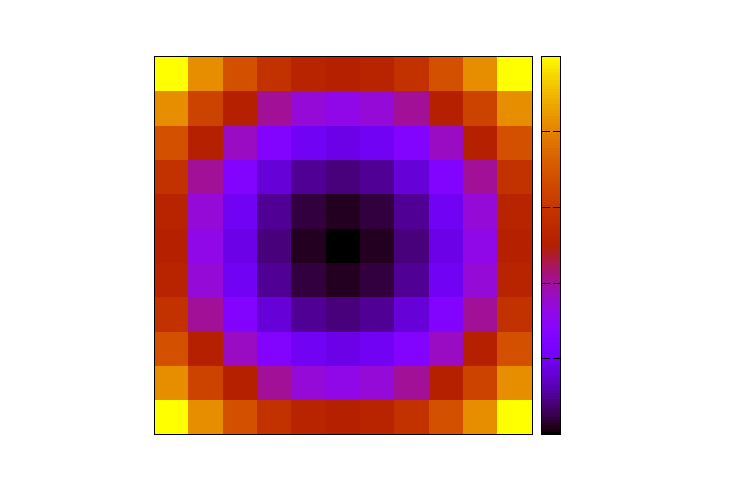
\includegraphics[width={360.00bp},height={237.00bp}]{test_heatmap}}%
    \gplfronttext
  \end{picture}%
\endgroup
}
  \resizebox{.48\linewidth}{!} {% GNUPLOT: LaTeX picture with Postscript
\begingroup
  \makeatletter
  \providecommand\color[2][]{%
    \GenericError{(gnuplot) \space\space\space\@spaces}{%
      Package color not loaded in conjunction with
      terminal option `colourtext'%
    }{See the gnuplot documentation for explanation.%
    }{Either use 'blacktext' in gnuplot or load the package
      color.sty in LaTeX.}%
    \renewcommand\color[2][]{}%
  }%
  \providecommand\includegraphics[2][]{%
    \GenericError{(gnuplot) \space\space\space\@spaces}{%
      Package graphicx or graphics not loaded%
    }{See the gnuplot documentation for explanation.%
    }{The gnuplot epslatex terminal needs graphicx.sty or graphics.sty.}%
    \renewcommand\includegraphics[2][]{}%
  }%
  \providecommand\rotatebox[2]{#2}%
  \@ifundefined{ifGPcolor}{%
    \newif\ifGPcolor
    \GPcolortrue
  }{}%
  \@ifundefined{ifGPblacktext}{%
    \newif\ifGPblacktext
    \GPblacktexttrue
  }{}%
  % define a \g@addto@macro without @ in the name:
  \let\gplgaddtomacro\g@addto@macro
  % define empty templates for all commands taking text:
  \gdef\gplbacktext{}%
  \gdef\gplfronttext{}%
  \makeatother
  \ifGPblacktext
    % no textcolor at all
    \def\colorrgb#1{}%
    \def\colorgray#1{}%
  \else
    % gray or color?
    \ifGPcolor
      \def\colorrgb#1{\color[rgb]{#1}}%
      \def\colorgray#1{\color[gray]{#1}}%
      \expandafter\def\csname LTw\endcsname{\color{white}}%
      \expandafter\def\csname LTb\endcsname{\color{black}}%
      \expandafter\def\csname LTa\endcsname{\color{black}}%
      \expandafter\def\csname LT0\endcsname{\color[rgb]{1,0,0}}%
      \expandafter\def\csname LT1\endcsname{\color[rgb]{0,1,0}}%
      \expandafter\def\csname LT2\endcsname{\color[rgb]{0,0,1}}%
      \expandafter\def\csname LT3\endcsname{\color[rgb]{1,0,1}}%
      \expandafter\def\csname LT4\endcsname{\color[rgb]{0,1,1}}%
      \expandafter\def\csname LT5\endcsname{\color[rgb]{1,1,0}}%
      \expandafter\def\csname LT6\endcsname{\color[rgb]{0,0,0}}%
      \expandafter\def\csname LT7\endcsname{\color[rgb]{1,0.3,0}}%
      \expandafter\def\csname LT8\endcsname{\color[rgb]{0.5,0.5,0.5}}%
    \else
      % gray
      \def\colorrgb#1{\color{black}}%
      \def\colorgray#1{\color[gray]{#1}}%
      \expandafter\def\csname LTw\endcsname{\color{white}}%
      \expandafter\def\csname LTb\endcsname{\color{black}}%
      \expandafter\def\csname LTa\endcsname{\color{black}}%
      \expandafter\def\csname LT0\endcsname{\color{black}}%
      \expandafter\def\csname LT1\endcsname{\color{black}}%
      \expandafter\def\csname LT2\endcsname{\color{black}}%
      \expandafter\def\csname LT3\endcsname{\color{black}}%
      \expandafter\def\csname LT4\endcsname{\color{black}}%
      \expandafter\def\csname LT5\endcsname{\color{black}}%
      \expandafter\def\csname LT6\endcsname{\color{black}}%
      \expandafter\def\csname LT7\endcsname{\color{black}}%
      \expandafter\def\csname LT8\endcsname{\color{black}}%
    \fi
  \fi
    \setlength{\unitlength}{0.0500bp}%
    \ifx\gptboxheight\undefined%
      \newlength{\gptboxheight}%
      \newlength{\gptboxwidth}%
      \newsavebox{\gptboxtext}%
    \fi%
    \setlength{\fboxrule}{0.5pt}%
    \setlength{\fboxsep}{1pt}%
    \definecolor{tbcol}{rgb}{1,1,1}%
\begin{picture}(7200.00,4740.00)%
    \gplgaddtomacro\gplbacktext{%
      \csname LTb\endcsname%%
      \put(932,1185){\makebox(0,0){\strut{}$0$}}%
      \csname LTb\endcsname%%
      \put(1402,1103){\makebox(0,0){\strut{}$5$}}%
      \csname LTb\endcsname%%
      \put(1872,1021){\makebox(0,0){\strut{}$10$}}%
      \csname LTb\endcsname%%
      \put(2342,939){\makebox(0,0){\strut{}$15$}}%
      \csname LTb\endcsname%%
      \put(2812,857){\makebox(0,0){\strut{}$20$}}%
      \csname LTb\endcsname%%
      \put(3282,775){\makebox(0,0){\strut{}$25$}}%
      \csname LTb\endcsname%%
      \put(3752,693){\makebox(0,0){\strut{}$30$}}%
      \csname LTb\endcsname%%
      \put(4222,611){\makebox(0,0){\strut{}$35$}}%
      \csname LTb\endcsname%%
      \put(4394,636){\makebox(0,0)[l]{\strut{}$-30$}}%
      \csname LTb\endcsname%%
      \put(4710,801){\makebox(0,0)[l]{\strut{}$-20$}}%
      \csname LTb\endcsname%%
      \put(5027,967){\makebox(0,0)[l]{\strut{}$-10$}}%
      \csname LTb\endcsname%%
      \put(5343,1133){\makebox(0,0)[l]{\strut{}$0$}}%
      \csname LTb\endcsname%%
      \put(5660,1298){\makebox(0,0)[l]{\strut{}$10$}}%
      \csname LTb\endcsname%%
      \put(5977,1464){\makebox(0,0)[l]{\strut{}$20$}}%
      \csname LTb\endcsname%%
      \put(6293,1630){\makebox(0,0)[l]{\strut{}$30$}}%
      \csname LTb\endcsname%%
      \put(854,1244){\makebox(0,0)[r]{\strut{}$-30$}}%
      \csname LTb\endcsname%%
      \put(854,1528){\makebox(0,0)[r]{\strut{}$-20$}}%
      \csname LTb\endcsname%%
      \put(854,1812){\makebox(0,0)[r]{\strut{}$-10$}}%
      \csname LTb\endcsname%%
      \put(854,2096){\makebox(0,0)[r]{\strut{}$0$}}%
      \csname LTb\endcsname%%
      \put(854,2379){\makebox(0,0)[r]{\strut{}$10$}}%
      \csname LTb\endcsname%%
      \put(854,2663){\makebox(0,0)[r]{\strut{}$20$}}%
      \csname LTb\endcsname%%
      \put(854,2947){\makebox(0,0)[r]{\strut{}$30$}}%
      \csname LTb\endcsname%%
      \put(854,3231){\makebox(0,0)[r]{\strut{}$40$}}%
    }%
    \gplgaddtomacro\gplfronttext{%
      \csname LTb\endcsname%%
      \put(6185,4297){\makebox(0,0)[r]{\strut{}points }}%
      \csname LTb\endcsname%%
      \put(2188,720){\makebox(0,0){\strut{}$x$}}%
      \csname LTb\endcsname%%
      \put(6018,1030){\makebox(0,0){\strut{}$xsin(x)$}}%
      \csname LTb\endcsname%%
      \put(310,2238){\makebox(0,0){\strut{}$xcos(x)$}}%
      \csname LTb\endcsname%%
      \put(6643,2110){\makebox(0,0)[l]{\strut{}$-30$}}%
      \csname LTb\endcsname%%
      \put(6643,2356){\makebox(0,0)[l]{\strut{}$-20$}}%
      \csname LTb\endcsname%%
      \put(6643,2603){\makebox(0,0)[l]{\strut{}$-10$}}%
      \csname LTb\endcsname%%
      \put(6643,2849){\makebox(0,0)[l]{\strut{}$0$}}%
      \csname LTb\endcsname%%
      \put(6643,3095){\makebox(0,0)[l]{\strut{}$10$}}%
      \csname LTb\endcsname%%
      \put(6643,3342){\makebox(0,0)[l]{\strut{}$20$}}%
      \csname LTb\endcsname%%
      \put(6643,3588){\makebox(0,0)[l]{\strut{}$30$}}%
      \csname LTb\endcsname%%
      \put(7132,2849){\rotatebox{-270}{\makebox(0,0){\strut{}$x/20$}}}%
    }%
    \gplbacktext
    \put(0,0){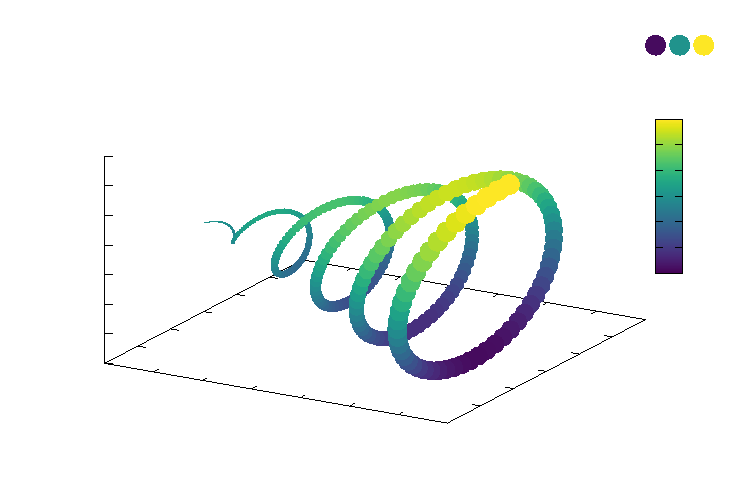
\includegraphics[width={360.00bp},height={237.00bp}]{test_line3d}}%
    \gplfronttext
  \end{picture}%
\endgroup
}

  \caption{Here it goes our nice caption explaining what all colours and lines are about. Note the mix of normal text and
  \LaTeX -like equations fonts.}
\end{figure}


\begin{figure}
  \resizebox{.48\linewidth}{!}{% GNUPLOT: LaTeX picture with Postscript
\begingroup
  \makeatletter
  \providecommand\color[2][]{%
    \GenericError{(gnuplot) \space\space\space\@spaces}{%
      Package color not loaded in conjunction with
      terminal option `colourtext'%
    }{See the gnuplot documentation for explanation.%
    }{Either use 'blacktext' in gnuplot or load the package
      color.sty in LaTeX.}%
    \renewcommand\color[2][]{}%
  }%
  \providecommand\includegraphics[2][]{%
    \GenericError{(gnuplot) \space\space\space\@spaces}{%
      Package graphicx or graphics not loaded%
    }{See the gnuplot documentation for explanation.%
    }{The gnuplot epslatex terminal needs graphicx.sty or graphics.sty.}%
    \renewcommand\includegraphics[2][]{}%
  }%
  \providecommand\rotatebox[2]{#2}%
  \@ifundefined{ifGPcolor}{%
    \newif\ifGPcolor
    \GPcolortrue
  }{}%
  \@ifundefined{ifGPblacktext}{%
    \newif\ifGPblacktext
    \GPblacktexttrue
  }{}%
  % define a \g@addto@macro without @ in the name:
  \let\gplgaddtomacro\g@addto@macro
  % define empty templates for all commands taking text:
  \gdef\gplbacktext{}%
  \gdef\gplfronttext{}%
  \makeatother
  \ifGPblacktext
    % no textcolor at all
    \def\colorrgb#1{}%
    \def\colorgray#1{}%
  \else
    % gray or color?
    \ifGPcolor
      \def\colorrgb#1{\color[rgb]{#1}}%
      \def\colorgray#1{\color[gray]{#1}}%
      \expandafter\def\csname LTw\endcsname{\color{white}}%
      \expandafter\def\csname LTb\endcsname{\color{black}}%
      \expandafter\def\csname LTa\endcsname{\color{black}}%
      \expandafter\def\csname LT0\endcsname{\color[rgb]{1,0,0}}%
      \expandafter\def\csname LT1\endcsname{\color[rgb]{0,1,0}}%
      \expandafter\def\csname LT2\endcsname{\color[rgb]{0,0,1}}%
      \expandafter\def\csname LT3\endcsname{\color[rgb]{1,0,1}}%
      \expandafter\def\csname LT4\endcsname{\color[rgb]{0,1,1}}%
      \expandafter\def\csname LT5\endcsname{\color[rgb]{1,1,0}}%
      \expandafter\def\csname LT6\endcsname{\color[rgb]{0,0,0}}%
      \expandafter\def\csname LT7\endcsname{\color[rgb]{1,0.3,0}}%
      \expandafter\def\csname LT8\endcsname{\color[rgb]{0.5,0.5,0.5}}%
    \else
      % gray
      \def\colorrgb#1{\color{black}}%
      \def\colorgray#1{\color[gray]{#1}}%
      \expandafter\def\csname LTw\endcsname{\color{white}}%
      \expandafter\def\csname LTb\endcsname{\color{black}}%
      \expandafter\def\csname LTa\endcsname{\color{black}}%
      \expandafter\def\csname LT0\endcsname{\color{black}}%
      \expandafter\def\csname LT1\endcsname{\color{black}}%
      \expandafter\def\csname LT2\endcsname{\color{black}}%
      \expandafter\def\csname LT3\endcsname{\color{black}}%
      \expandafter\def\csname LT4\endcsname{\color{black}}%
      \expandafter\def\csname LT5\endcsname{\color{black}}%
      \expandafter\def\csname LT6\endcsname{\color{black}}%
      \expandafter\def\csname LT7\endcsname{\color{black}}%
      \expandafter\def\csname LT8\endcsname{\color{black}}%
    \fi
  \fi
    \setlength{\unitlength}{0.0500bp}%
    \ifx\gptboxheight\undefined%
      \newlength{\gptboxheight}%
      \newlength{\gptboxwidth}%
      \newsavebox{\gptboxtext}%
    \fi%
    \setlength{\fboxrule}{0.5pt}%
    \setlength{\fboxsep}{1pt}%
    \definecolor{tbcol}{rgb}{1,1,1}%
\begin{picture}(7200.00,4740.00)%
    \gplgaddtomacro\gplbacktext{%
      \csname LTb\endcsname%%
      \put(616,562){\makebox(0,0)[r]{\strut{}$0$}}%
      \csname LTb\endcsname%%
      \put(616,1321){\makebox(0,0)[r]{\strut{}$20$}}%
      \csname LTb\endcsname%%
      \put(616,2079){\makebox(0,0)[r]{\strut{}$40$}}%
      \csname LTb\endcsname%%
      \put(616,2837){\makebox(0,0)[r]{\strut{}$60$}}%
      \csname LTb\endcsname%%
      \put(616,3596){\makebox(0,0)[r]{\strut{}$80$}}%
      \csname LTb\endcsname%%
      \put(616,4354){\makebox(0,0)[r]{\strut{}$100$}}%
      \csname LTb\endcsname%%
      \put(714,386){\makebox(0,0){\strut{}$0$}}%
      \csname LTb\endcsname%%
      \put(1889,386){\makebox(0,0){\strut{}$2$}}%
      \csname LTb\endcsname%%
      \put(3065,386){\makebox(0,0){\strut{}$4$}}%
      \csname LTb\endcsname%%
      \put(4241,386){\makebox(0,0){\strut{}$6$}}%
      \csname LTb\endcsname%%
      \put(5416,386){\makebox(0,0){\strut{}$8$}}%
      \csname LTb\endcsname%%
      \put(6592,386){\makebox(0,0){\strut{}$10$}}%
    }%
    \gplgaddtomacro\gplfronttext{%
      \csname LTb\endcsname%%
      \put(161,2553){\rotatebox{-270}{\makebox(0,0){\strut{}$y$}}}%
      \csname LTb\endcsname%%
      \put(3800,123){\makebox(0,0){\strut{}$x$}}%
      \csname LTb\endcsname%%
      \put(1008,4385){\makebox(0,0)[r]{\strut{}1}}%
      \csname LTb\endcsname%%
      \put(1008,4209){\makebox(0,0)[r]{\strut{}2}}%
      \csname LTb\endcsname%%
      \put(1008,4033){\makebox(0,0)[r]{\strut{}3}}%
      \csname LTb\endcsname%%
      \put(1008,3858){\makebox(0,0)[r]{\strut{}4}}%
      \csname LTb\endcsname%%
      \put(1008,3682){\makebox(0,0)[r]{\strut{}5}}%
      \csname LTb\endcsname%%
      \put(1008,3506){\makebox(0,0)[r]{\strut{}6}}%
      \csname LTb\endcsname%%
      \put(1008,3330){\makebox(0,0)[r]{\strut{}7}}%
      \csname LTb\endcsname%%
      \put(1008,3154){\makebox(0,0)[r]{\strut{}8}}%
      \csname LTb\endcsname%%
      \put(1008,2978){\makebox(0,0)[r]{\strut{}9}}%
      \csname LTb\endcsname%%
      \put(1008,2802){\makebox(0,0)[r]{\strut{}10}}%
    }%
    \gplbacktext
    \put(0,0){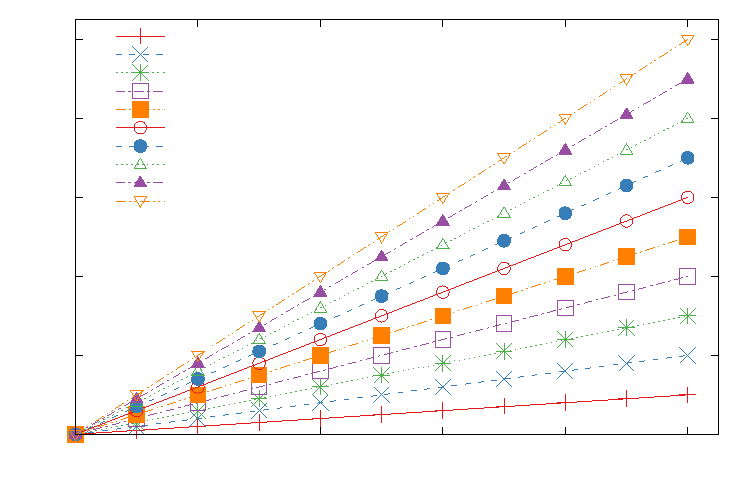
\includegraphics[width={360.00bp},height={237.00bp}]{test_ls}}%
    \gplfronttext
  \end{picture}%
\endgroup
}
  \resizebox{.48\linewidth}{!}{% GNUPLOT: LaTeX picture with Postscript
\begingroup
  \makeatletter
  \providecommand\color[2][]{%
    \GenericError{(gnuplot) \space\space\space\@spaces}{%
      Package color not loaded in conjunction with
      terminal option `colourtext'%
    }{See the gnuplot documentation for explanation.%
    }{Either use 'blacktext' in gnuplot or load the package
      color.sty in LaTeX.}%
    \renewcommand\color[2][]{}%
  }%
  \providecommand\includegraphics[2][]{%
    \GenericError{(gnuplot) \space\space\space\@spaces}{%
      Package graphicx or graphics not loaded%
    }{See the gnuplot documentation for explanation.%
    }{The gnuplot epslatex terminal needs graphicx.sty or graphics.sty.}%
    \renewcommand\includegraphics[2][]{}%
  }%
  \providecommand\rotatebox[2]{#2}%
  \@ifundefined{ifGPcolor}{%
    \newif\ifGPcolor
    \GPcolortrue
  }{}%
  \@ifundefined{ifGPblacktext}{%
    \newif\ifGPblacktext
    \GPblacktexttrue
  }{}%
  % define a \g@addto@macro without @ in the name:
  \let\gplgaddtomacro\g@addto@macro
  % define empty templates for all commands taking text:
  \gdef\gplbacktext{}%
  \gdef\gplfronttext{}%
  \makeatother
  \ifGPblacktext
    % no textcolor at all
    \def\colorrgb#1{}%
    \def\colorgray#1{}%
  \else
    % gray or color?
    \ifGPcolor
      \def\colorrgb#1{\color[rgb]{#1}}%
      \def\colorgray#1{\color[gray]{#1}}%
      \expandafter\def\csname LTw\endcsname{\color{white}}%
      \expandafter\def\csname LTb\endcsname{\color{black}}%
      \expandafter\def\csname LTa\endcsname{\color{black}}%
      \expandafter\def\csname LT0\endcsname{\color[rgb]{1,0,0}}%
      \expandafter\def\csname LT1\endcsname{\color[rgb]{0,1,0}}%
      \expandafter\def\csname LT2\endcsname{\color[rgb]{0,0,1}}%
      \expandafter\def\csname LT3\endcsname{\color[rgb]{1,0,1}}%
      \expandafter\def\csname LT4\endcsname{\color[rgb]{0,1,1}}%
      \expandafter\def\csname LT5\endcsname{\color[rgb]{1,1,0}}%
      \expandafter\def\csname LT6\endcsname{\color[rgb]{0,0,0}}%
      \expandafter\def\csname LT7\endcsname{\color[rgb]{1,0.3,0}}%
      \expandafter\def\csname LT8\endcsname{\color[rgb]{0.5,0.5,0.5}}%
    \else
      % gray
      \def\colorrgb#1{\color{black}}%
      \def\colorgray#1{\color[gray]{#1}}%
      \expandafter\def\csname LTw\endcsname{\color{white}}%
      \expandafter\def\csname LTb\endcsname{\color{black}}%
      \expandafter\def\csname LTa\endcsname{\color{black}}%
      \expandafter\def\csname LT0\endcsname{\color{black}}%
      \expandafter\def\csname LT1\endcsname{\color{black}}%
      \expandafter\def\csname LT2\endcsname{\color{black}}%
      \expandafter\def\csname LT3\endcsname{\color{black}}%
      \expandafter\def\csname LT4\endcsname{\color{black}}%
      \expandafter\def\csname LT5\endcsname{\color{black}}%
      \expandafter\def\csname LT6\endcsname{\color{black}}%
      \expandafter\def\csname LT7\endcsname{\color{black}}%
      \expandafter\def\csname LT8\endcsname{\color{black}}%
    \fi
  \fi
    \setlength{\unitlength}{0.0500bp}%
    \ifx\gptboxheight\undefined%
      \newlength{\gptboxheight}%
      \newlength{\gptboxwidth}%
      \newsavebox{\gptboxtext}%
    \fi%
    \setlength{\fboxrule}{0.5pt}%
    \setlength{\fboxsep}{1pt}%
    \definecolor{tbcol}{rgb}{1,1,1}%
\begin{picture}(7200.00,4740.00)%
    \gplgaddtomacro\gplbacktext{%
      \csname LTb\endcsname%%
      \put(620,899){\makebox(0,0)[r]{\strut{}$-0.2$}}%
      \csname LTb\endcsname%%
      \put(620,1663){\makebox(0,0)[r]{\strut{}$0$}}%
      \csname LTb\endcsname%%
      \put(620,2428){\makebox(0,0)[r]{\strut{}$0.2$}}%
      \csname LTb\endcsname%%
      \put(620,3193){\makebox(0,0)[r]{\strut{}$0.4$}}%
      \csname LTb\endcsname%%
      \put(620,3957){\makebox(0,0)[r]{\strut{}$0.6$}}%
      \csname LTb\endcsname%%
      \put(1029,610){\rotatebox{-35}{\makebox(0,0)[l]{\strut{}2018-01-11}}}%
      \csname LTb\endcsname%%
      \put(1464,610){\rotatebox{-35}{\makebox(0,0)[l]{\strut{}2018-01-25}}}%
      \csname LTb\endcsname%%
      \put(1900,610){\rotatebox{-35}{\makebox(0,0)[l]{\strut{}2018-02-08}}}%
      \csname LTb\endcsname%%
      \put(2335,610){\rotatebox{-35}{\makebox(0,0)[l]{\strut{}2018-02-22}}}%
      \csname LTb\endcsname%%
      \put(2771,610){\rotatebox{-35}{\makebox(0,0)[l]{\strut{}2018-03-08}}}%
      \csname LTb\endcsname%%
      \put(3207,610){\rotatebox{-35}{\makebox(0,0)[l]{\strut{}2018-03-22}}}%
    }%
    \gplgaddtomacro\gplfronttext{%
    }%
    \gplgaddtomacro\gplbacktext{%
      \csname LTb\endcsname%%
      \put(3635,899){\makebox(0,0)[r]{\strut{}}}%
      \csname LTb\endcsname%%
      \put(3635,1663){\makebox(0,0)[r]{\strut{}}}%
      \csname LTb\endcsname%%
      \put(3635,2428){\makebox(0,0)[r]{\strut{}}}%
      \csname LTb\endcsname%%
      \put(3635,3193){\makebox(0,0)[r]{\strut{}}}%
      \csname LTb\endcsname%%
      \put(3635,3957){\makebox(0,0)[r]{\strut{}}}%
      \csname LTb\endcsname%%
      \put(3743,610){\rotatebox{-35}{\makebox(0,0)[l]{\strut{}2018-07-01}}}%
      \csname LTb\endcsname%%
      \put(4208,610){\rotatebox{-35}{\makebox(0,0)[l]{\strut{}2018-08-01}}}%
      \csname LTb\endcsname%%
      \put(4689,610){\rotatebox{-35}{\makebox(0,0)[l]{\strut{}2018-09-01}}}%
      \csname LTb\endcsname%%
      \put(5155,610){\rotatebox{-35}{\makebox(0,0)[l]{\strut{}2018-10-01}}}%
      \csname LTb\endcsname%%
      \put(5621,610){\rotatebox{-35}{\makebox(0,0)[l]{\strut{}2018-11-01}}}%
      \csname LTb\endcsname%%
      \put(6086,610){\rotatebox{-35}{\makebox(0,0)[l]{\strut{}2018-12-01}}}%
    }%
    \gplgaddtomacro\gplfronttext{%
      \csname LTb\endcsname%%
      \put(5778,4372){\makebox(0,0)[r]{\strut{}series}}%
    }%
    \gplbacktext
    \put(0,0){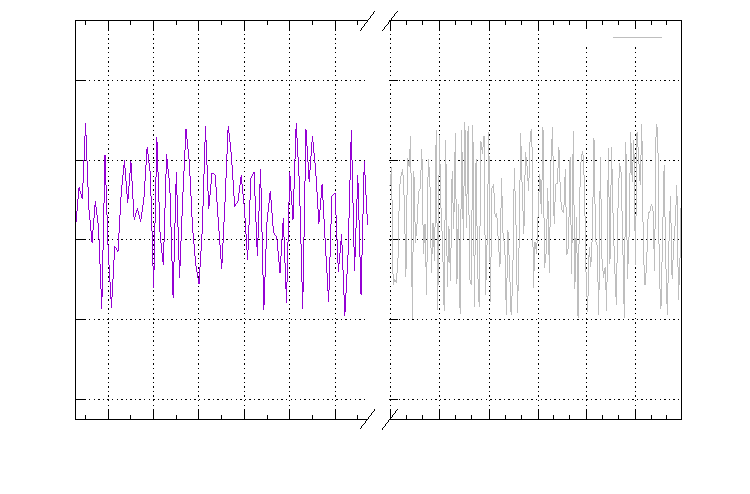
\includegraphics[width={360.00bp},height={237.00bp}]{test_dates}}%
    \gplfronttext
  \end{picture}%
\endgroup
}
  \caption{Here it goes our nice caption explaining what all colours and lines are about. Note the mix of normal text and
  \LaTeX -like equations fonts.}
\end{figure}

\begin{figure}
\resizebox{.48\linewidth}{!} {% GNUPLOT: LaTeX picture with Postscript
\begingroup
  \makeatletter
  \providecommand\color[2][]{%
    \GenericError{(gnuplot) \space\space\space\@spaces}{%
      Package color not loaded in conjunction with
      terminal option `colourtext'%
    }{See the gnuplot documentation for explanation.%
    }{Either use 'blacktext' in gnuplot or load the package
      color.sty in LaTeX.}%
    \renewcommand\color[2][]{}%
  }%
  \providecommand\includegraphics[2][]{%
    \GenericError{(gnuplot) \space\space\space\@spaces}{%
      Package graphicx or graphics not loaded%
    }{See the gnuplot documentation for explanation.%
    }{The gnuplot epslatex terminal needs graphicx.sty or graphics.sty.}%
    \renewcommand\includegraphics[2][]{}%
  }%
  \providecommand\rotatebox[2]{#2}%
  \@ifundefined{ifGPcolor}{%
    \newif\ifGPcolor
    \GPcolortrue
  }{}%
  \@ifundefined{ifGPblacktext}{%
    \newif\ifGPblacktext
    \GPblacktexttrue
  }{}%
  % define a \g@addto@macro without @ in the name:
  \let\gplgaddtomacro\g@addto@macro
  % define empty templates for all commands taking text:
  \gdef\gplbacktext{}%
  \gdef\gplfronttext{}%
  \makeatother
  \ifGPblacktext
    % no textcolor at all
    \def\colorrgb#1{}%
    \def\colorgray#1{}%
  \else
    % gray or color?
    \ifGPcolor
      \def\colorrgb#1{\color[rgb]{#1}}%
      \def\colorgray#1{\color[gray]{#1}}%
      \expandafter\def\csname LTw\endcsname{\color{white}}%
      \expandafter\def\csname LTb\endcsname{\color{black}}%
      \expandafter\def\csname LTa\endcsname{\color{black}}%
      \expandafter\def\csname LT0\endcsname{\color[rgb]{1,0,0}}%
      \expandafter\def\csname LT1\endcsname{\color[rgb]{0,1,0}}%
      \expandafter\def\csname LT2\endcsname{\color[rgb]{0,0,1}}%
      \expandafter\def\csname LT3\endcsname{\color[rgb]{1,0,1}}%
      \expandafter\def\csname LT4\endcsname{\color[rgb]{0,1,1}}%
      \expandafter\def\csname LT5\endcsname{\color[rgb]{1,1,0}}%
      \expandafter\def\csname LT6\endcsname{\color[rgb]{0,0,0}}%
      \expandafter\def\csname LT7\endcsname{\color[rgb]{1,0.3,0}}%
      \expandafter\def\csname LT8\endcsname{\color[rgb]{0.5,0.5,0.5}}%
    \else
      % gray
      \def\colorrgb#1{\color{black}}%
      \def\colorgray#1{\color[gray]{#1}}%
      \expandafter\def\csname LTw\endcsname{\color{white}}%
      \expandafter\def\csname LTb\endcsname{\color{black}}%
      \expandafter\def\csname LTa\endcsname{\color{black}}%
      \expandafter\def\csname LT0\endcsname{\color{black}}%
      \expandafter\def\csname LT1\endcsname{\color{black}}%
      \expandafter\def\csname LT2\endcsname{\color{black}}%
      \expandafter\def\csname LT3\endcsname{\color{black}}%
      \expandafter\def\csname LT4\endcsname{\color{black}}%
      \expandafter\def\csname LT5\endcsname{\color{black}}%
      \expandafter\def\csname LT6\endcsname{\color{black}}%
      \expandafter\def\csname LT7\endcsname{\color{black}}%
      \expandafter\def\csname LT8\endcsname{\color{black}}%
    \fi
  \fi
    \setlength{\unitlength}{0.0500bp}%
    \ifx\gptboxheight\undefined%
      \newlength{\gptboxheight}%
      \newlength{\gptboxwidth}%
      \newsavebox{\gptboxtext}%
    \fi%
    \setlength{\fboxrule}{0.5pt}%
    \setlength{\fboxsep}{1pt}%
    \definecolor{tbcol}{rgb}{1,1,1}%
\begin{picture}(7200.00,7200.00)%
    \gplgaddtomacro\gplbacktext{%
    }%
    \gplgaddtomacro\gplfronttext{%
      \csname LTb\endcsname%%
      \put(1219,183){\makebox(0,0){\strut{}$0$}}%
      \csname LTb\endcsname%%
      \put(1886,183){\makebox(0,0){\strut{}$500$}}%
      \csname LTb\endcsname%%
      \put(2553,183){\makebox(0,0){\strut{}$1000$}}%
      \csname LTb\endcsname%%
      \put(3219,183){\makebox(0,0){\strut{}$1500$}}%
      \csname LTb\endcsname%%
      \put(3886,183){\makebox(0,0){\strut{}$2000$}}%
      \csname LTb\endcsname%%
      \put(4553,183){\makebox(0,0){\strut{}$2500$}}%
      \csname LTb\endcsname%%
      \put(5220,183){\makebox(0,0){\strut{}$3000$}}%
      \csname LTb\endcsname%%
      \put(5887,183){\makebox(0,0){\strut{}$3500$}}%
      \csname LTb\endcsname%%
      \put(3554,0){\makebox(0,0){\strut{}GPP}}%
      \csname LTb\endcsname%%
      \put(3590,6838){\makebox(0,0){\strut{}Gross Primary Production}}%
    }%
    \gplbacktext
    \put(0,0){\includegraphics[width={360.00bp},height={360.00bp}]{test_gpp}}%
    \gplfronttext
  \end{picture}%
\endgroup
}
  \resizebox{.48\linewidth}{!} {\textcolor{white}{
  {% GNUPLOT: LaTeX picture with Postscript
\begingroup
  \makeatletter
  \providecommand\color[2][]{%
    \GenericError{(gnuplot) \space\space\space\@spaces}{%
      Package color not loaded in conjunction with
      terminal option `colourtext'%
    }{See the gnuplot documentation for explanation.%
    }{Either use 'blacktext' in gnuplot or load the package
      color.sty in LaTeX.}%
    \renewcommand\color[2][]{}%
  }%
  \providecommand\includegraphics[2][]{%
    \GenericError{(gnuplot) \space\space\space\@spaces}{%
      Package graphicx or graphics not loaded%
    }{See the gnuplot documentation for explanation.%
    }{The gnuplot epslatex terminal needs graphicx.sty or graphics.sty.}%
    \renewcommand\includegraphics[2][]{}%
  }%
  \providecommand\rotatebox[2]{#2}%
  \@ifundefined{ifGPcolor}{%
    \newif\ifGPcolor
    \GPcolortrue
  }{}%
  \@ifundefined{ifGPblacktext}{%
    \newif\ifGPblacktext
    \GPblacktexttrue
  }{}%
  % define a \g@addto@macro without @ in the name:
  \let\gplgaddtomacro\g@addto@macro
  % define empty templates for all commands taking text:
  \gdef\gplbacktext{}%
  \gdef\gplfronttext{}%
  \makeatother
  \ifGPblacktext
    % no textcolor at all
    \def\colorrgb#1{}%
    \def\colorgray#1{}%
  \else
    % gray or color?
    \ifGPcolor
      \def\colorrgb#1{\color[rgb]{#1}}%
      \def\colorgray#1{\color[gray]{#1}}%
      \expandafter\def\csname LTw\endcsname{\color{white}}%
      \expandafter\def\csname LTb\endcsname{\color{black}}%
      \expandafter\def\csname LTa\endcsname{\color{black}}%
      \expandafter\def\csname LT0\endcsname{\color[rgb]{1,0,0}}%
      \expandafter\def\csname LT1\endcsname{\color[rgb]{0,1,0}}%
      \expandafter\def\csname LT2\endcsname{\color[rgb]{0,0,1}}%
      \expandafter\def\csname LT3\endcsname{\color[rgb]{1,0,1}}%
      \expandafter\def\csname LT4\endcsname{\color[rgb]{0,1,1}}%
      \expandafter\def\csname LT5\endcsname{\color[rgb]{1,1,0}}%
      \expandafter\def\csname LT6\endcsname{\color[rgb]{0,0,0}}%
      \expandafter\def\csname LT7\endcsname{\color[rgb]{1,0.3,0}}%
      \expandafter\def\csname LT8\endcsname{\color[rgb]{0.5,0.5,0.5}}%
    \else
      % gray
      \def\colorrgb#1{\color{black}}%
      \def\colorgray#1{\color[gray]{#1}}%
      \expandafter\def\csname LTw\endcsname{\color{white}}%
      \expandafter\def\csname LTb\endcsname{\color{black}}%
      \expandafter\def\csname LTa\endcsname{\color{black}}%
      \expandafter\def\csname LT0\endcsname{\color{black}}%
      \expandafter\def\csname LT1\endcsname{\color{black}}%
      \expandafter\def\csname LT2\endcsname{\color{black}}%
      \expandafter\def\csname LT3\endcsname{\color{black}}%
      \expandafter\def\csname LT4\endcsname{\color{black}}%
      \expandafter\def\csname LT5\endcsname{\color{black}}%
      \expandafter\def\csname LT6\endcsname{\color{black}}%
      \expandafter\def\csname LT7\endcsname{\color{black}}%
      \expandafter\def\csname LT8\endcsname{\color{black}}%
    \fi
  \fi
    \setlength{\unitlength}{0.0500bp}%
    \ifx\gptboxheight\undefined%
      \newlength{\gptboxheight}%
      \newlength{\gptboxwidth}%
      \newsavebox{\gptboxtext}%
    \fi%
    \setlength{\fboxrule}{0.5pt}%
    \setlength{\fboxsep}{1pt}%
    \definecolor{tbcol}{rgb}{1,1,1}%
\begin{picture}(7200.00,7200.00)%
    \gplgaddtomacro\gplbacktext{%
    }%
    \gplgaddtomacro\gplfronttext{%
      \colorrgb{1.00,1.00,1.00}%%
      \put(1220,398){\makebox(0,0){\strut{}$-6000$}}%
      \colorrgb{1.00,1.00,1.00}%%
      \put(1998,398){\makebox(0,0){\strut{}$-4000$}}%
      \colorrgb{1.00,1.00,1.00}%%
      \put(2776,398){\makebox(0,0){\strut{}$-2000$}}%
      \colorrgb{1.00,1.00,1.00}%%
      \put(3554,398){\makebox(0,0){\strut{}$0$}}%
      \colorrgb{1.00,1.00,1.00}%%
      \put(4331,398){\makebox(0,0){\strut{}$2000$}}%
      \colorrgb{1.00,1.00,1.00}%%
      \put(5109,398){\makebox(0,0){\strut{}$4000$}}%
      \colorrgb{1.00,1.00,1.00}%%
      \put(5887,398){\makebox(0,0){\strut{}$6000$}}%
      \colorrgb{1.00,1.00,1.00}%%
      \put(3554,99){\makebox(0,0){\strut{}$m$}}%
      \csname LTb\endcsname%%
      \put(5740,6228){\makebox(0,0){\strut{}\color{white} $G_{\mu\nu} + \Lambda g_{\mu\nu} = \kappa T_{\mu\nu}$}}%
      \csname LTb\endcsname%%
      \put(3590,6760){\makebox(0,0){\strut{}\color{white} ETOPO Global Relief Model}}%
    }%
    \gplbacktext
    \put(0,0){\includegraphics[width={360.00bp},height={360.00bp}]{test_topo}}%
    \gplfronttext
  \end{picture}%
\endgroup

  }}}\\
  {\footnotesize
% GNUPLOT: LaTeX picture with Postscript
\begingroup
  \makeatletter
  \providecommand\color[2][]{%
    \GenericError{(gnuplot) \space\space\space\@spaces}{%
      Package color not loaded in conjunction with
      terminal option `colourtext'%
    }{See the gnuplot documentation for explanation.%
    }{Either use 'blacktext' in gnuplot or load the package
      color.sty in LaTeX.}%
    \renewcommand\color[2][]{}%
  }%
  \providecommand\includegraphics[2][]{%
    \GenericError{(gnuplot) \space\space\space\@spaces}{%
      Package graphicx or graphics not loaded%
    }{See the gnuplot documentation for explanation.%
    }{The gnuplot epslatex terminal needs graphicx.sty or graphics.sty.}%
    \renewcommand\includegraphics[2][]{}%
  }%
  \providecommand\rotatebox[2]{#2}%
  \@ifundefined{ifGPcolor}{%
    \newif\ifGPcolor
    \GPcolortrue
  }{}%
  \@ifundefined{ifGPblacktext}{%
    \newif\ifGPblacktext
    \GPblacktexttrue
  }{}%
  % define a \g@addto@macro without @ in the name:
  \let\gplgaddtomacro\g@addto@macro
  % define empty templates for all commands taking text:
  \gdef\gplbacktext{}%
  \gdef\gplfronttext{}%
  \makeatother
  \ifGPblacktext
    % no textcolor at all
    \def\colorrgb#1{}%
    \def\colorgray#1{}%
  \else
    % gray or color?
    \ifGPcolor
      \def\colorrgb#1{\color[rgb]{#1}}%
      \def\colorgray#1{\color[gray]{#1}}%
      \expandafter\def\csname LTw\endcsname{\color{white}}%
      \expandafter\def\csname LTb\endcsname{\color{black}}%
      \expandafter\def\csname LTa\endcsname{\color{black}}%
      \expandafter\def\csname LT0\endcsname{\color[rgb]{1,0,0}}%
      \expandafter\def\csname LT1\endcsname{\color[rgb]{0,1,0}}%
      \expandafter\def\csname LT2\endcsname{\color[rgb]{0,0,1}}%
      \expandafter\def\csname LT3\endcsname{\color[rgb]{1,0,1}}%
      \expandafter\def\csname LT4\endcsname{\color[rgb]{0,1,1}}%
      \expandafter\def\csname LT5\endcsname{\color[rgb]{1,1,0}}%
      \expandafter\def\csname LT6\endcsname{\color[rgb]{0,0,0}}%
      \expandafter\def\csname LT7\endcsname{\color[rgb]{1,0.3,0}}%
      \expandafter\def\csname LT8\endcsname{\color[rgb]{0.5,0.5,0.5}}%
    \else
      % gray
      \def\colorrgb#1{\color{black}}%
      \def\colorgray#1{\color[gray]{#1}}%
      \expandafter\def\csname LTw\endcsname{\color{white}}%
      \expandafter\def\csname LTb\endcsname{\color{black}}%
      \expandafter\def\csname LTa\endcsname{\color{black}}%
      \expandafter\def\csname LT0\endcsname{\color{black}}%
      \expandafter\def\csname LT1\endcsname{\color{black}}%
      \expandafter\def\csname LT2\endcsname{\color{black}}%
      \expandafter\def\csname LT3\endcsname{\color{black}}%
      \expandafter\def\csname LT4\endcsname{\color{black}}%
      \expandafter\def\csname LT5\endcsname{\color{black}}%
      \expandafter\def\csname LT6\endcsname{\color{black}}%
      \expandafter\def\csname LT7\endcsname{\color{black}}%
      \expandafter\def\csname LT8\endcsname{\color{black}}%
    \fi
  \fi
    \setlength{\unitlength}{0.0500bp}%
    \ifx\gptboxheight\undefined%
      \newlength{\gptboxheight}%
      \newlength{\gptboxwidth}%
      \newsavebox{\gptboxtext}%
    \fi%
    \setlength{\fboxrule}{0.5pt}%
    \setlength{\fboxsep}{1pt}%
    \definecolor{tbcol}{rgb}{1,1,1}%
\begin{picture}(8640.00,2160.00)%
    \gplgaddtomacro\gplbacktext{%
      \csname LTb\endcsname%%
      \put(714,562){\makebox(0,0)[r]{\strut{}$-1$}}%
      \csname LTb\endcsname%%
      \put(714,913){\makebox(0,0)[r]{\strut{}$-0.5$}}%
      \csname LTb\endcsname%%
      \put(714,1263){\makebox(0,0)[r]{\strut{}$0$}}%
      \csname LTb\endcsname%%
      \put(714,1613){\makebox(0,0)[r]{\strut{}$0.5$}}%
      \csname LTb\endcsname%%
      \put(714,1964){\makebox(0,0)[r]{\strut{}$1$}}%
      \csname LTb\endcsname%%
      \put(812,386){\makebox(0,0){\strut{}$0.01$}}%
      \csname LTb\endcsname%%
      \put(2427,386){\makebox(0,0){\strut{}$0.1$}}%
      \csname LTb\endcsname%%
      \put(4041,386){\makebox(0,0){\strut{}$1$}}%
      \csname LTb\endcsname%%
      \put(5656,386){\makebox(0,0){\strut{}$10$}}%
      \csname LTb\endcsname%%
      \put(7271,386){\makebox(0,0){\strut{}$100$}}%
    }%
    \gplgaddtomacro\gplfronttext{%
      \csname LTb\endcsname%%
      \put(161,1263){\rotatebox{-270}{\makebox(0,0){\strut{}$-0.75sin(x)$}}}%
      \csname LTb\endcsname%%
      \put(4041,123){\makebox(0,0){\strut{}default format $x$}}%
      \csname LTb\endcsname%%
      \put(7853,562){\makebox(0,0)[l]{\strut{}$10^{-2}$}}%
      \csname LTb\endcsname%%
      \put(7853,913){\makebox(0,0)[l]{\strut{}$10^{-1}$}}%
      \csname LTb\endcsname%%
      \put(7853,1263){\makebox(0,0)[l]{\strut{}$10^{0}$}}%
      \csname LTb\endcsname%%
      \put(7853,1613){\makebox(0,0)[l]{\strut{}$10^{1}$}}%
      \csname LTb\endcsname%%
      \put(7853,1964){\makebox(0,0)[l]{\strut{}$10^{2}$}}%
      \csname LTb\endcsname%%
      \put(8294,1263){\rotatebox{-270}{\makebox(0,0){\strut{}Scientific Notation}}}%
    }%
    \gplbacktext
    \put(0,0){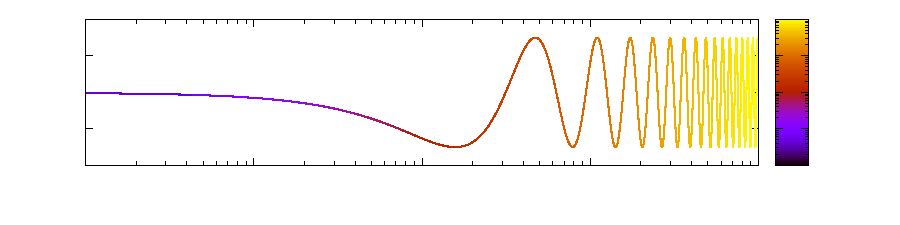
\includegraphics[width={432.00bp},height={108.00bp}]{test_log}}%
    \gplfronttext
  \end{picture}%
\endgroup

}
  \caption{Here it goes our nice caption explaining what all colours and lines are about. Note the mix of normal text and
  \LaTeX -like equations fonts.}
\end{figure}

\end{document}